%\section{Results}
Figure \ref{fig:cross_section_model} shows the differential cross sections \xsecproton as a function of \QSqproton for C, Fe, and Pb in data. The GENIE FSI and the NuWro FSI models (with 2p2h and RPA correction included by both generators) are compared to the data.  Predictions from each of these generators without FSI are also compared to the data. As shown previously by Fig. 3, the FSI treatments are needed to achieve agreement. The data exhibits an $A$-dependence and better agreement with NuWro than GENIE; at higher $A$ the protons move to lower energy, suggesting an increase in  proton energy loss in the nucleus. The measurement tests the FSI treatments,  especially with respect to pion absorption and proton inelastic scattering. NuWro has medium effects for pion absorption FSI that give a strong dependence on $A$, effects that are not included in GENIE.

The consequences of incorporating 2p2h events and RPA kinematic distortion into the GENIE simulation were evaluated. Adding the 2p2h reaction to the default GENIE model changes the predicted cross section by 20\% for C, 21\% for Fe, and 22\% for Pb. Adding the RPA produces a $0.6\%$ change because the most affected events are below the proton tracking threshold of this analysis. Neither the 2p2h nor the RPA model predicts significant $A$ dependence.
The chi-square between the GENIE simulation, with and without 2p2h and RPA, and the data is shown in Table \ref{tab:model_compare}, together with the chi-square for NuWro with 2p2h plus RPA compared to the data.
\begin{figure}[htpb]
\centering
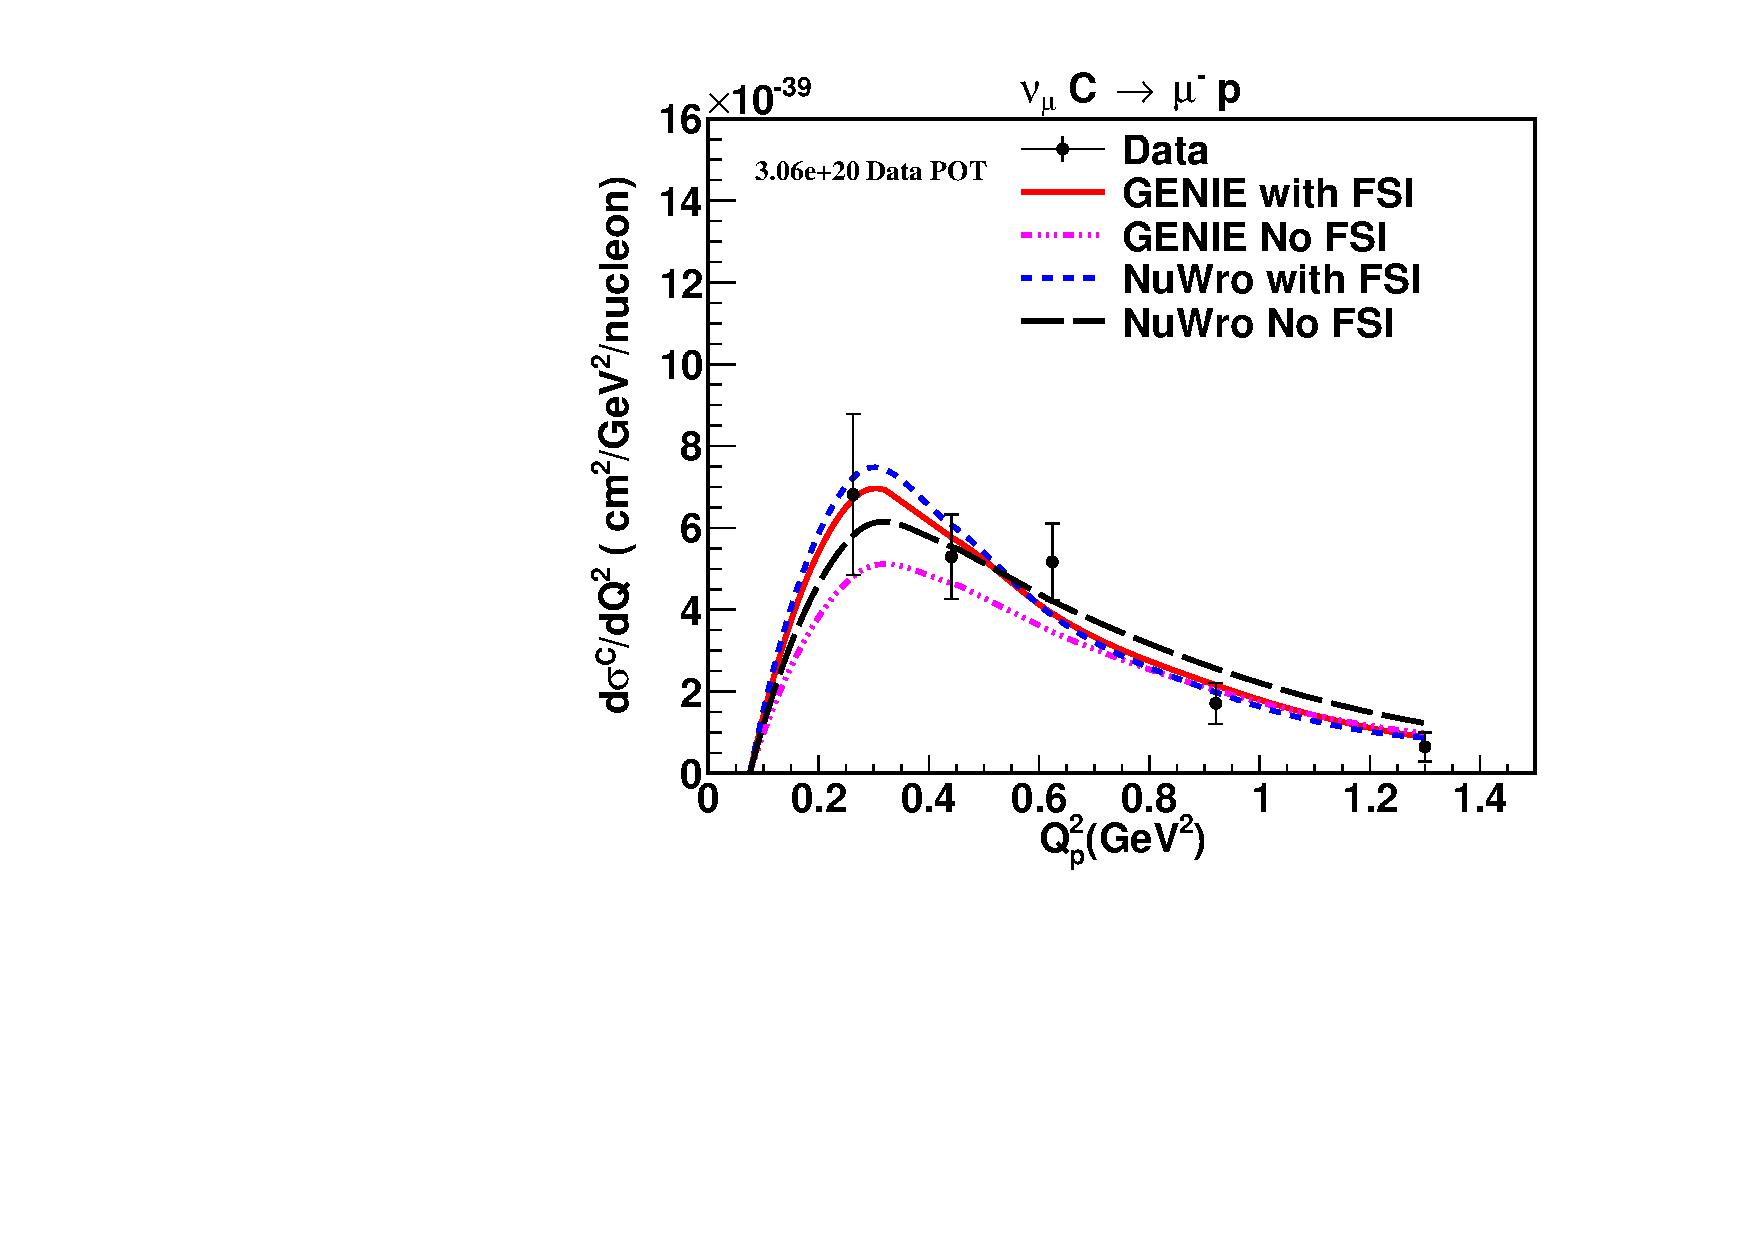
\includegraphics[trim = 0mm 4mm 10mm 2mm, clip, width=0.48\columnwidth]{DiffXsec_C.pdf}
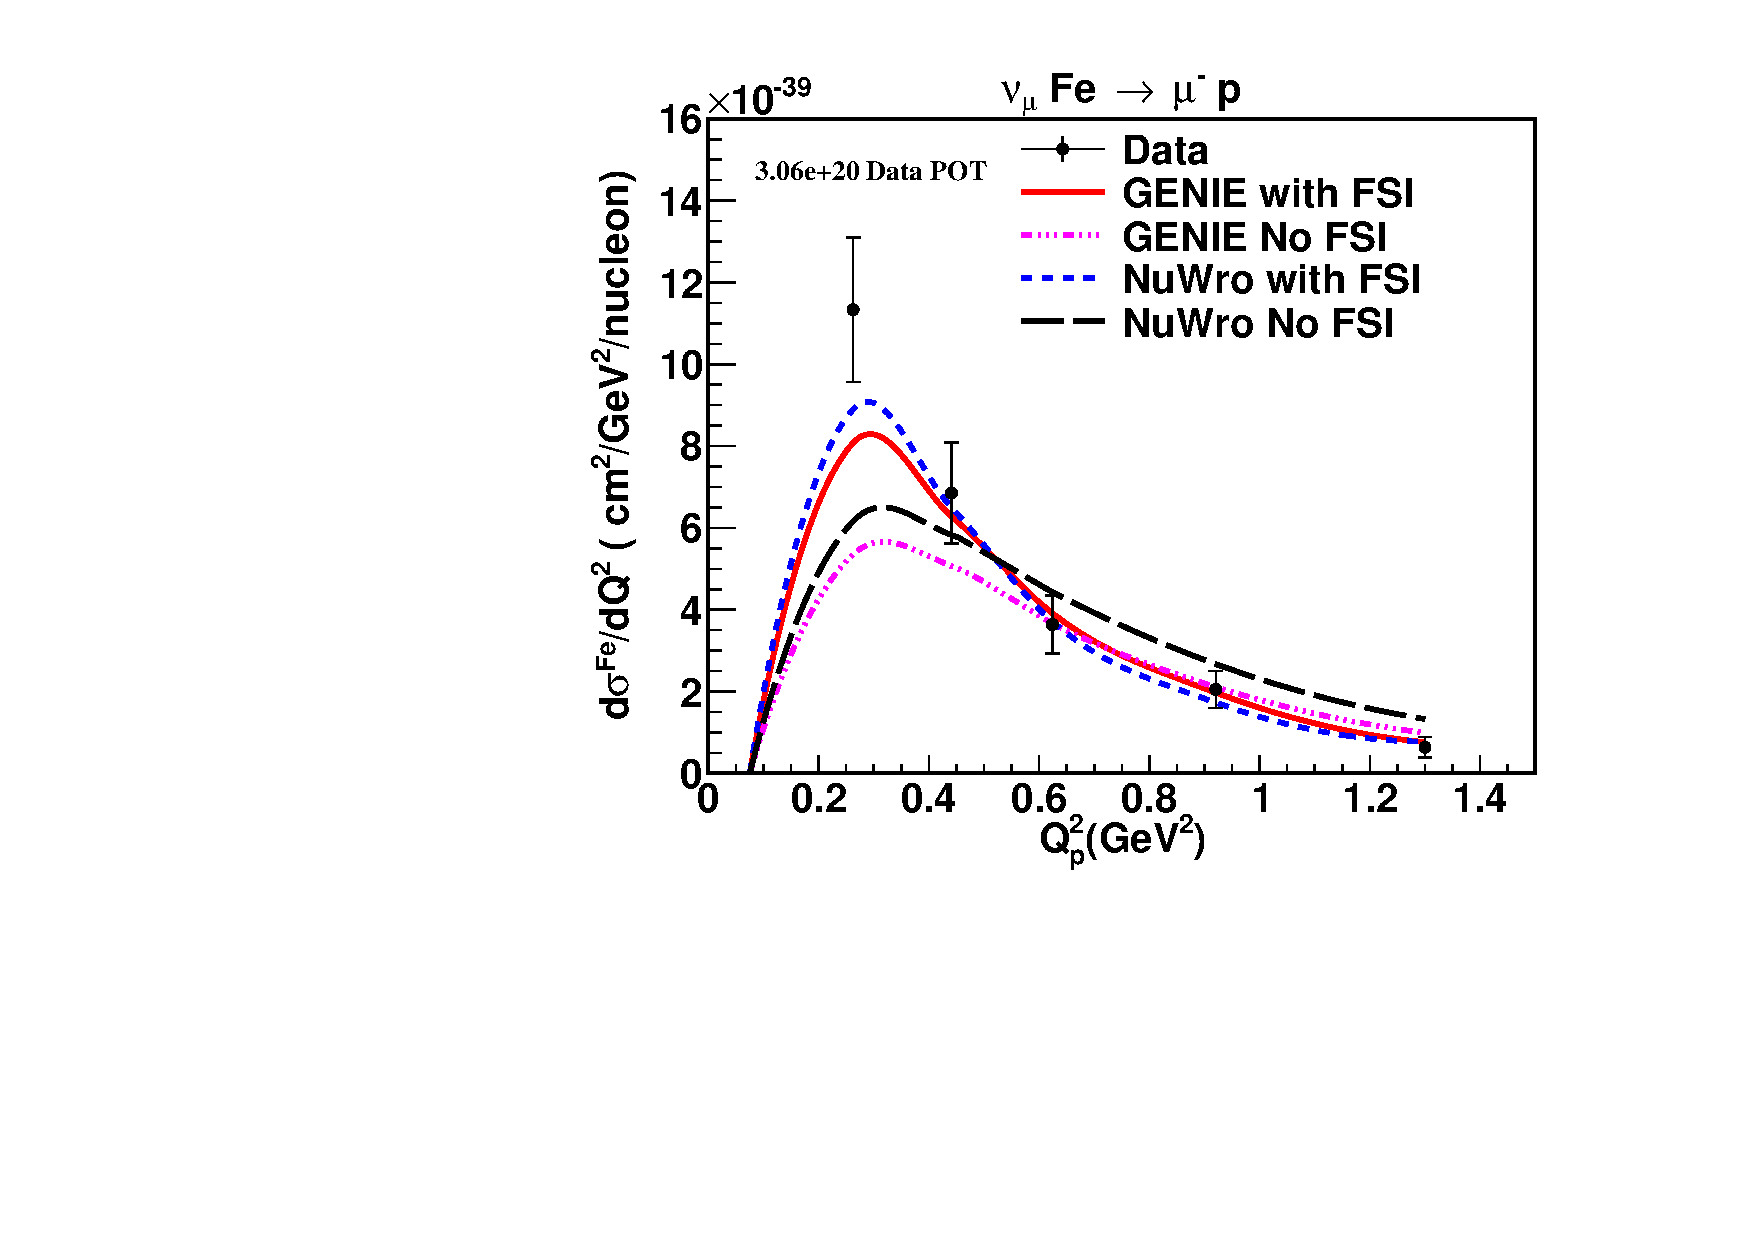
\includegraphics[trim = 0mm 4mm 10mm 2mm, clip, width=0.48\columnwidth]{DiffXsec_Fe.pdf}
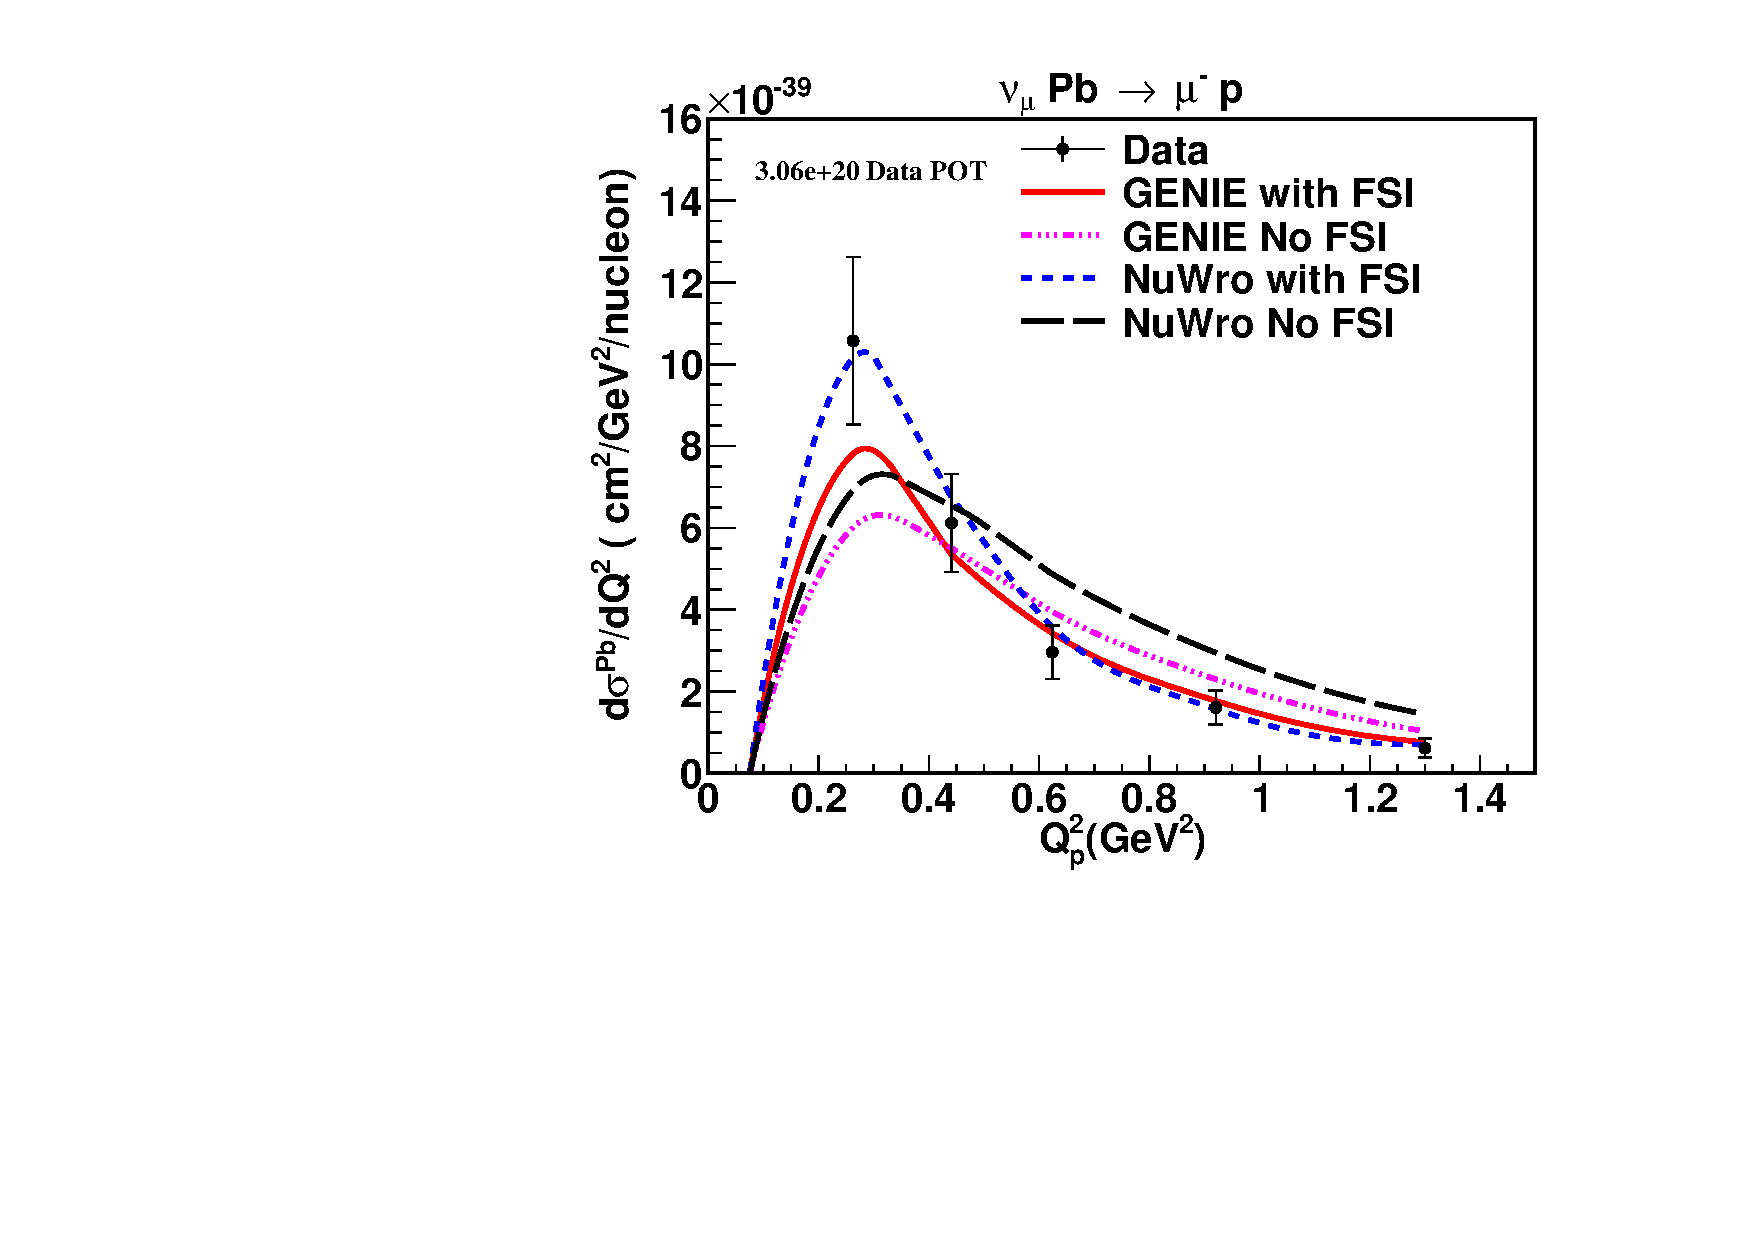
\includegraphics[trim = 0mm 4mm 10mm 2mm, clip, width=0.48\columnwidth]{DiffXsec_Pb.pdf}
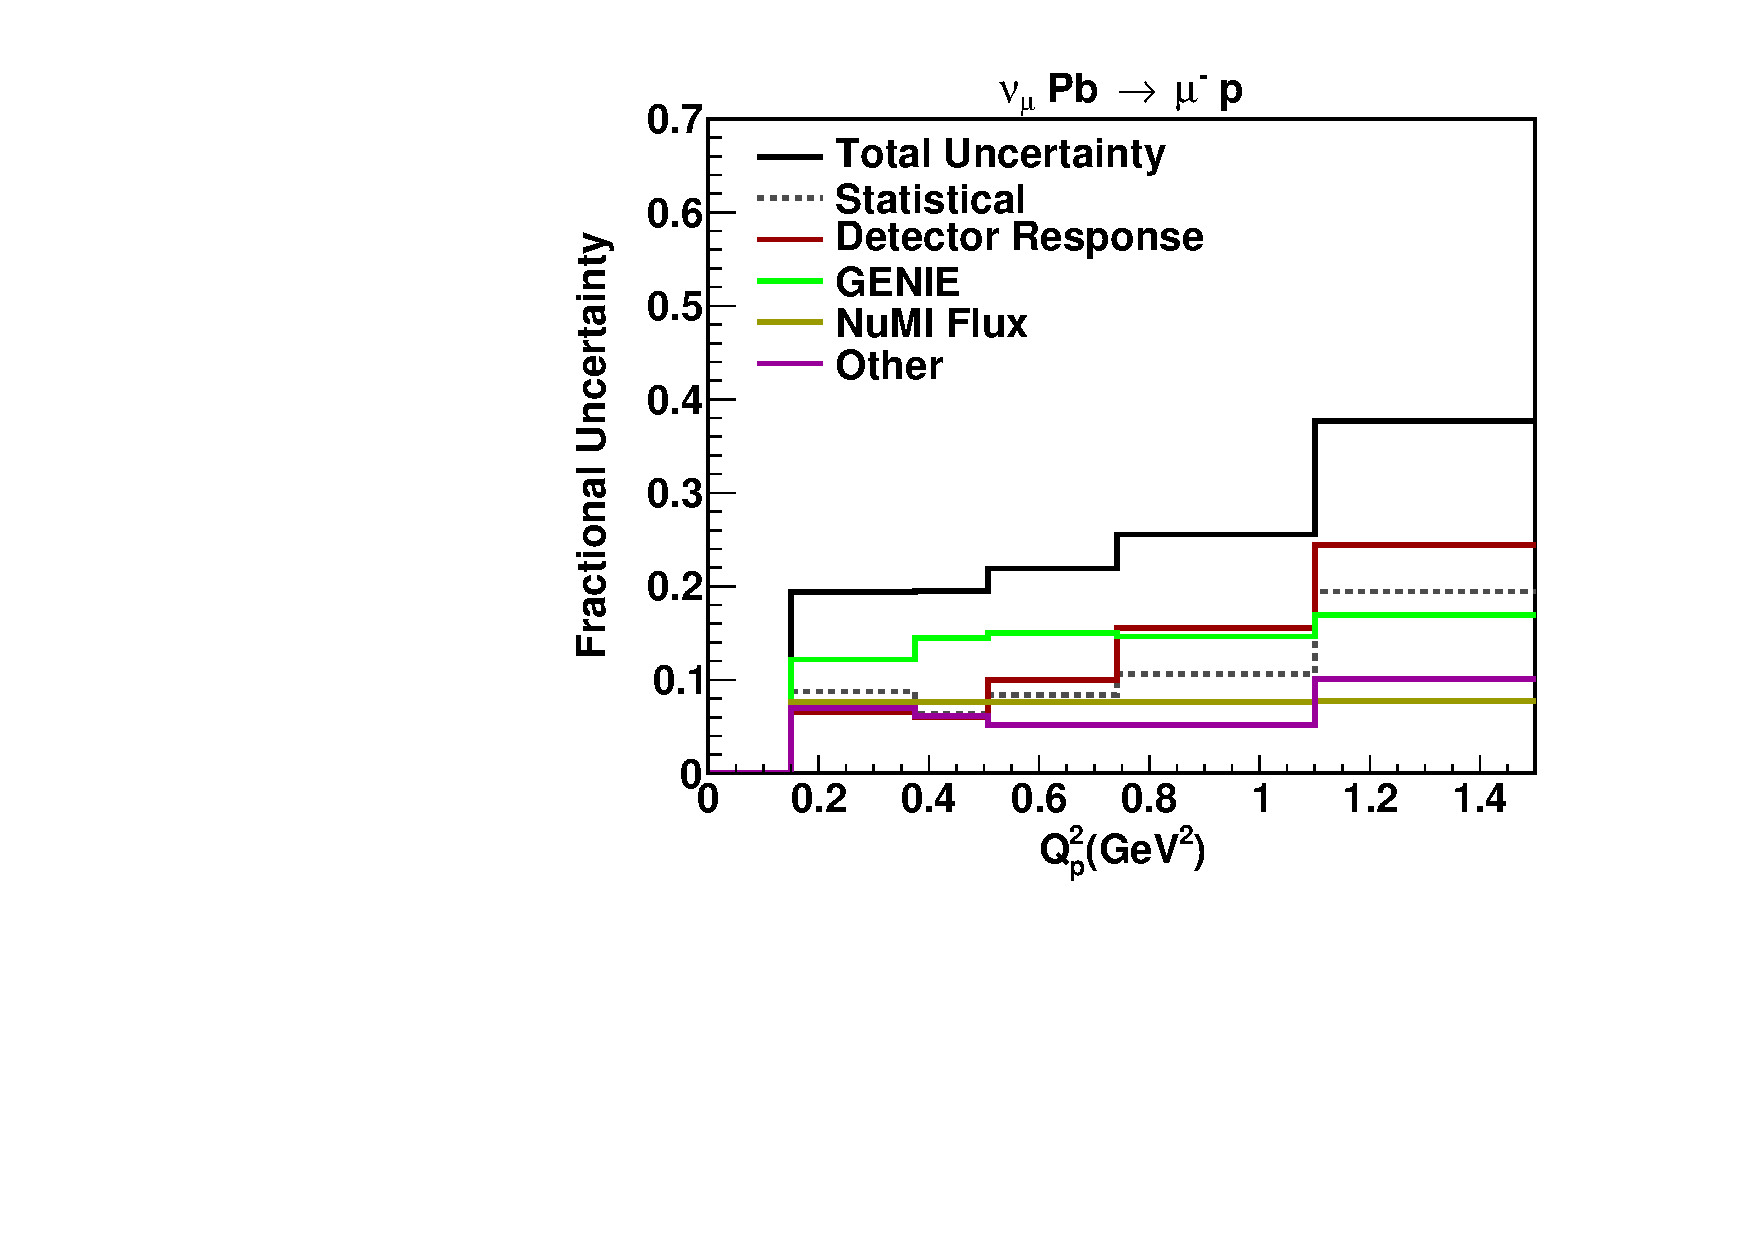
\includegraphics[trim = 0mm 4mm 10mm 2mm, width=0.48\columnwidth]{DiffXsec_PbError.pdf}
\caption{ Differential cross sections as a function of $Q^{2}$ for C (top-left), Fe (top-right) and Pb (bottom-left) compared to predictions from \genie and \nuwro which include 2p2h and RPA. The bottom right plot shows the fractional uncertainties for $\frac{d\sigma}{dQ^{2}_{p}}$ of Pb; the dashed curve is from statistical and the solid curves show systematic uncertainties for each of the contributions.}\label{fig:cross_section_model}
\end{figure}


\begin{table}[!htbp]
\centering
\caption{Calculated $\chi^{2}$ between the data and various models with M$_{A}$ = 0.99~ GeV.
The number of degrees of freedom is 5.\label{tab:model_compare}}
\scalebox{0.8}
{
\begin{tabular}{ l c c c }
               Model & Carbon   & Iron & Lead \\ \hline
\genie  RFG              & 11.0 & 63.8 & 41.1   \\
\genie  RFG + 2p2h       & 5.9  & 18.9 & 16.3   \\
\genie RFG + 2p2h + RPA  & 5.9  & 19.9 & 17.5   \\
\nuwro RFG + 2p2h + RPA  & 6.0  & 14.6 & 11.0   \\
\end{tabular}
}
\end{table}
Figure \ref{fig:ratios} shows the ratios of $\frac{d\sigma}{dQ^{2}_{p}}$ on C, Fe and Pb to the same quantity as measured in the high statistics CH sample.  The data ratios are helped by reduction of systematics uncertainties including the flux. The data ratios emphasize the increasingly strong effect on C, Fe and Pb. The model ratios show that a large effect can be attributed to FSI and is similar for both GENIE and NuWro.  In addition,  NuWro better describes the lowest $Q^2_p$ points with its $A$-dependent pion absorption model and medium corrections. In the $\QSqproton<0.6$ GeV$^2$ region, GENIE predicts that $28\%$ of CCQE-like signal events are from the pion absorption process.
 The coplanarity angle also shows an $A$ dependence, which may partially be from FSI.   
\begin{figure}[htpb]
\centering
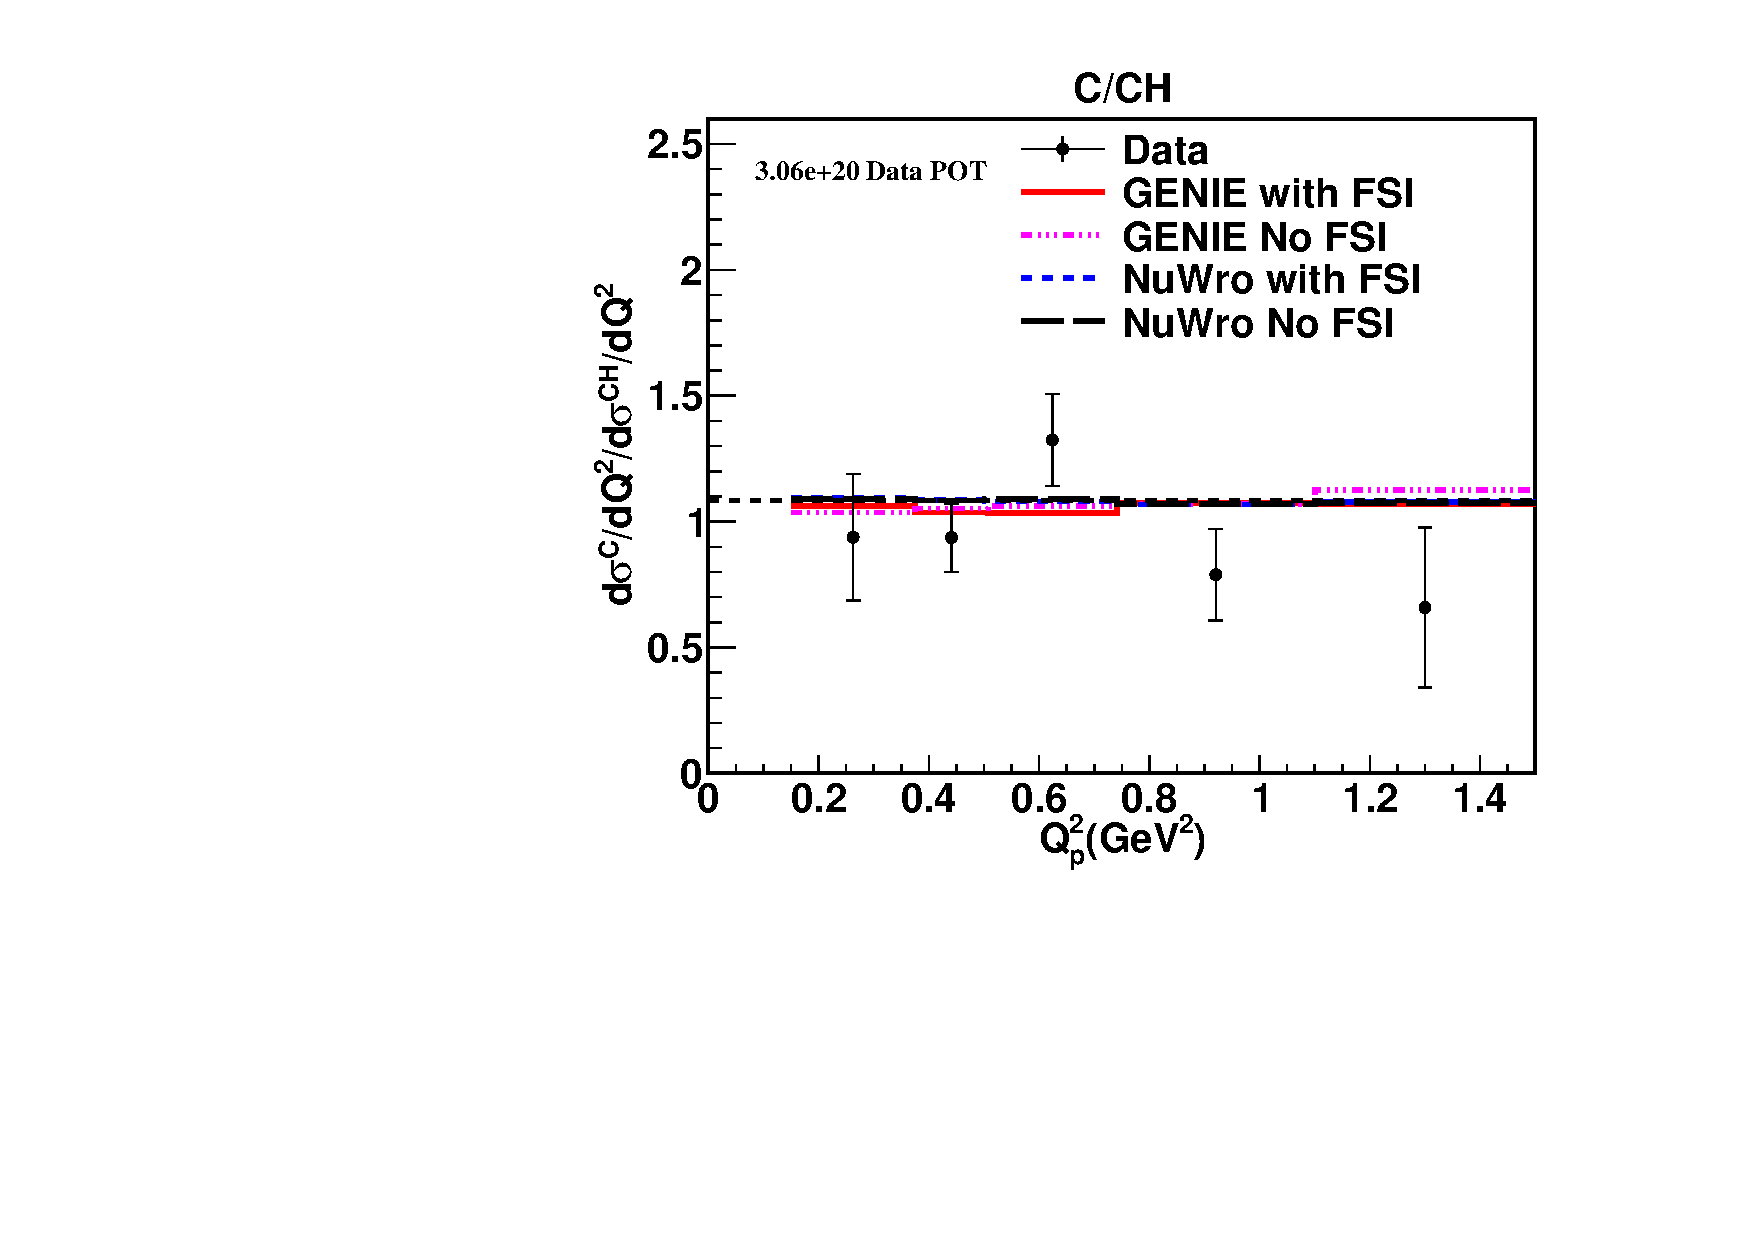
\includegraphics[trim = 0mm 4mm 10mm 2mm, clip, width=0.48\columnwidth]{Ratio_C.pdf}
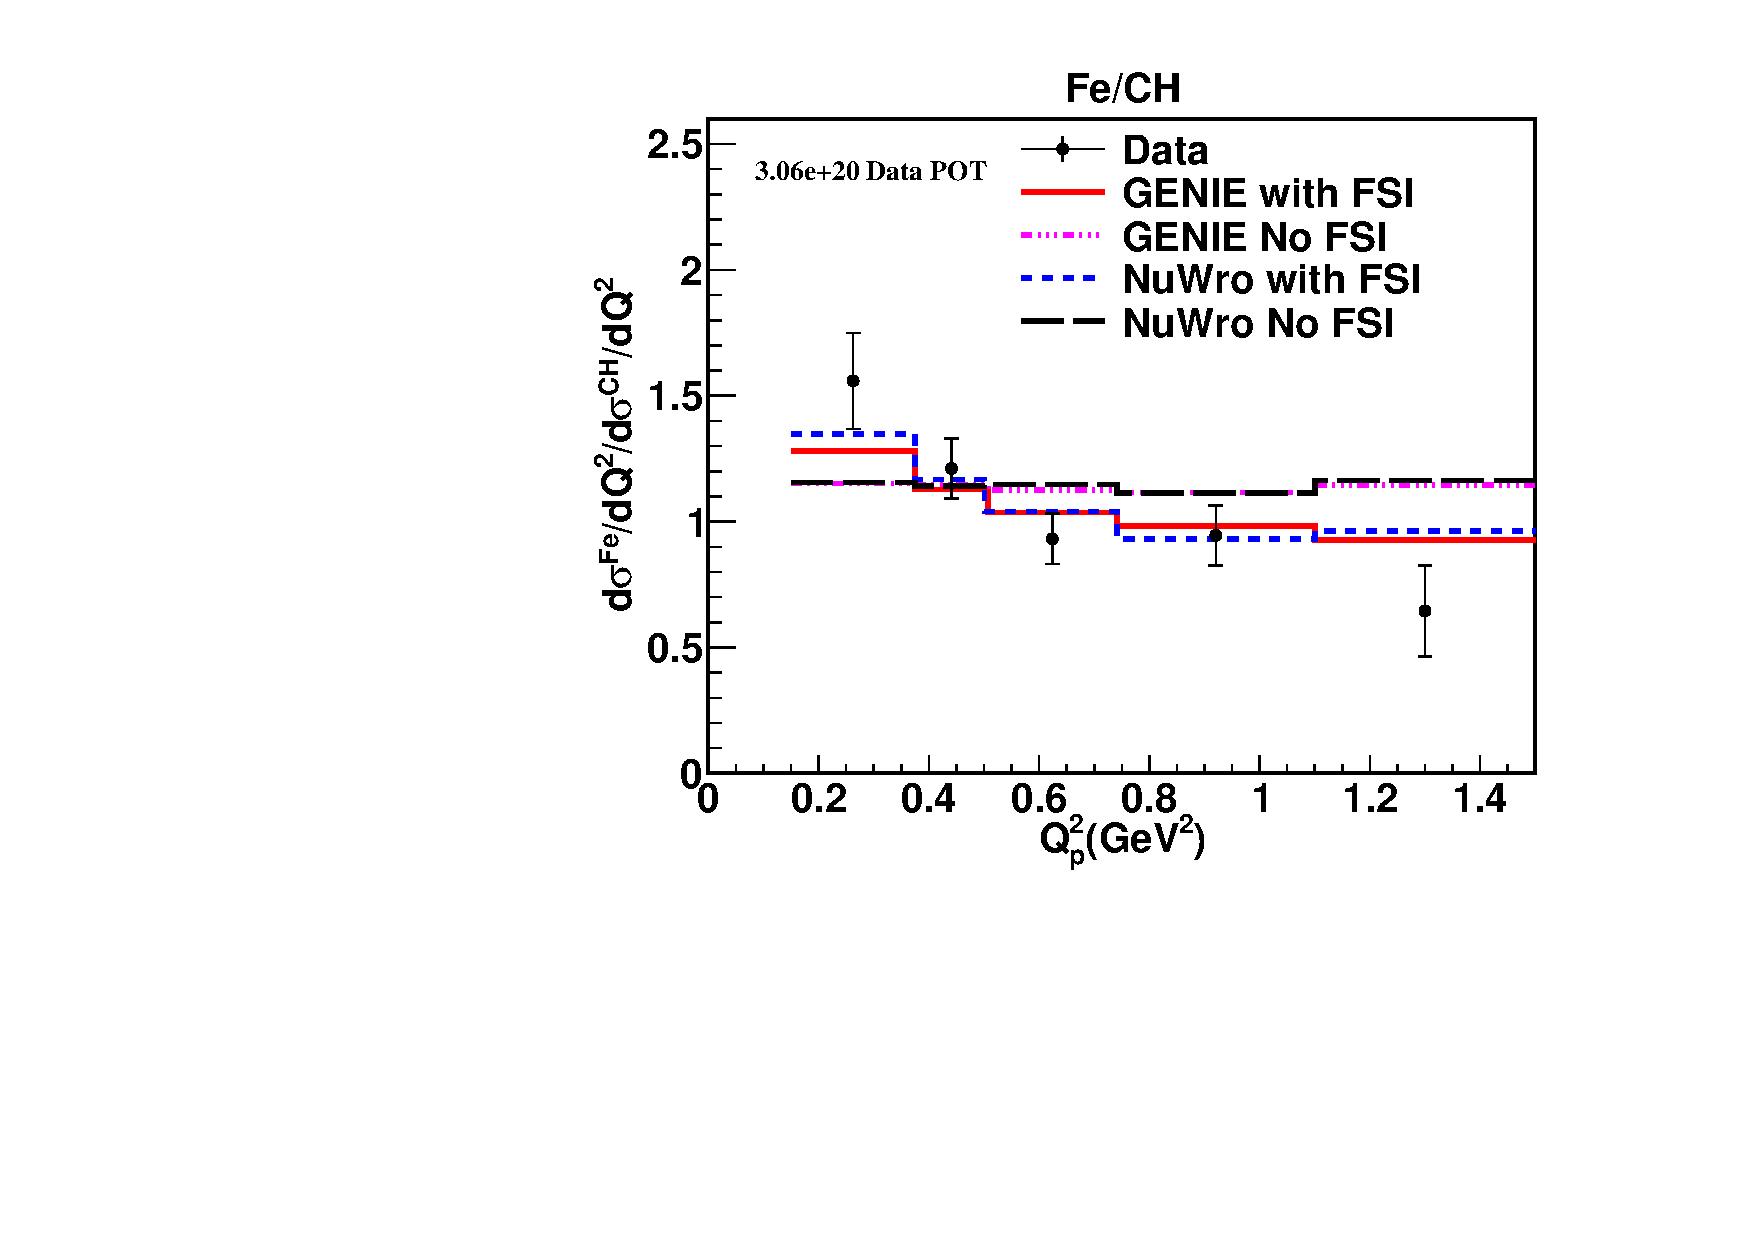
\includegraphics[trim = 0mm 4mm 10mm 2mm, clip, width=0.48\columnwidth]{Ratio_Fe.pdf}
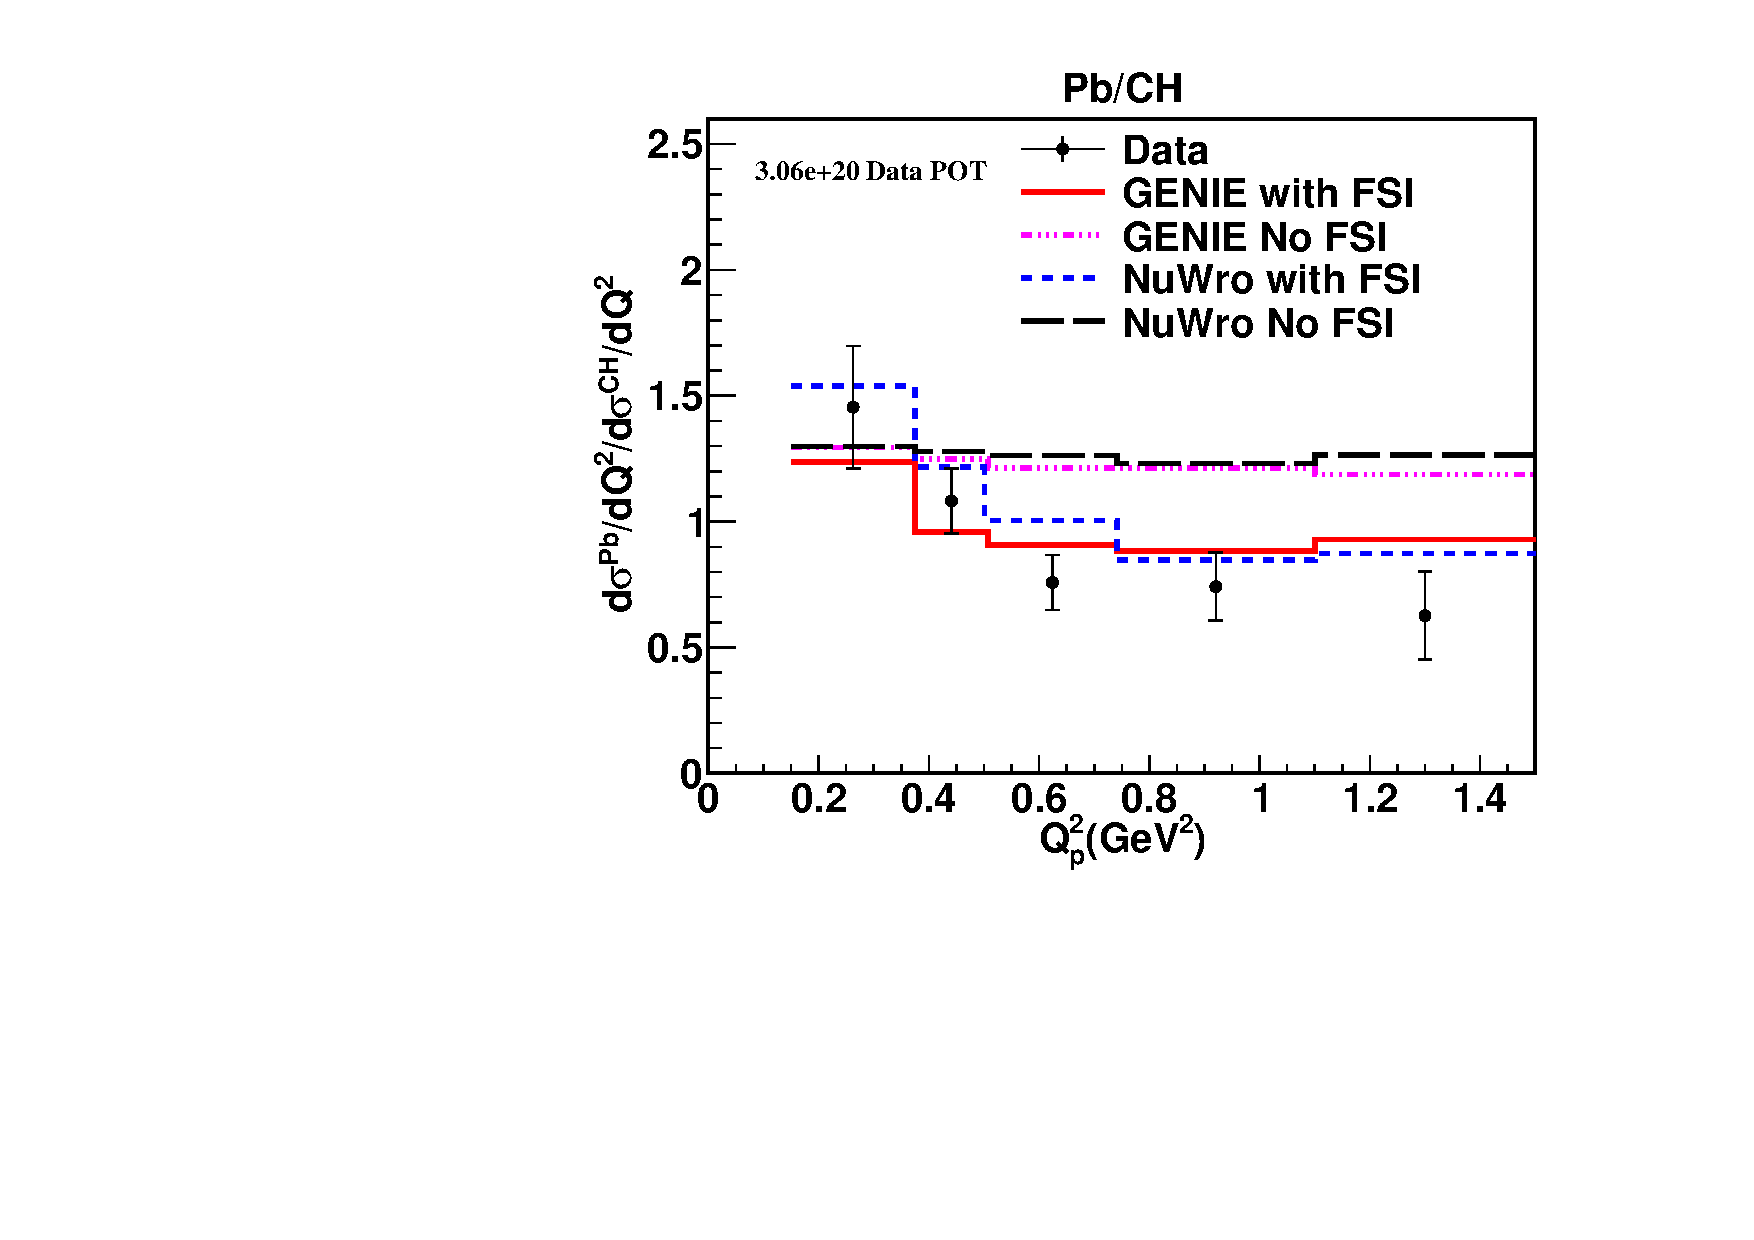
\includegraphics[trim = 0mm 4mm 10mm 2mm, clip, width=0.48\columnwidth]{Ratio_Pb.pdf}
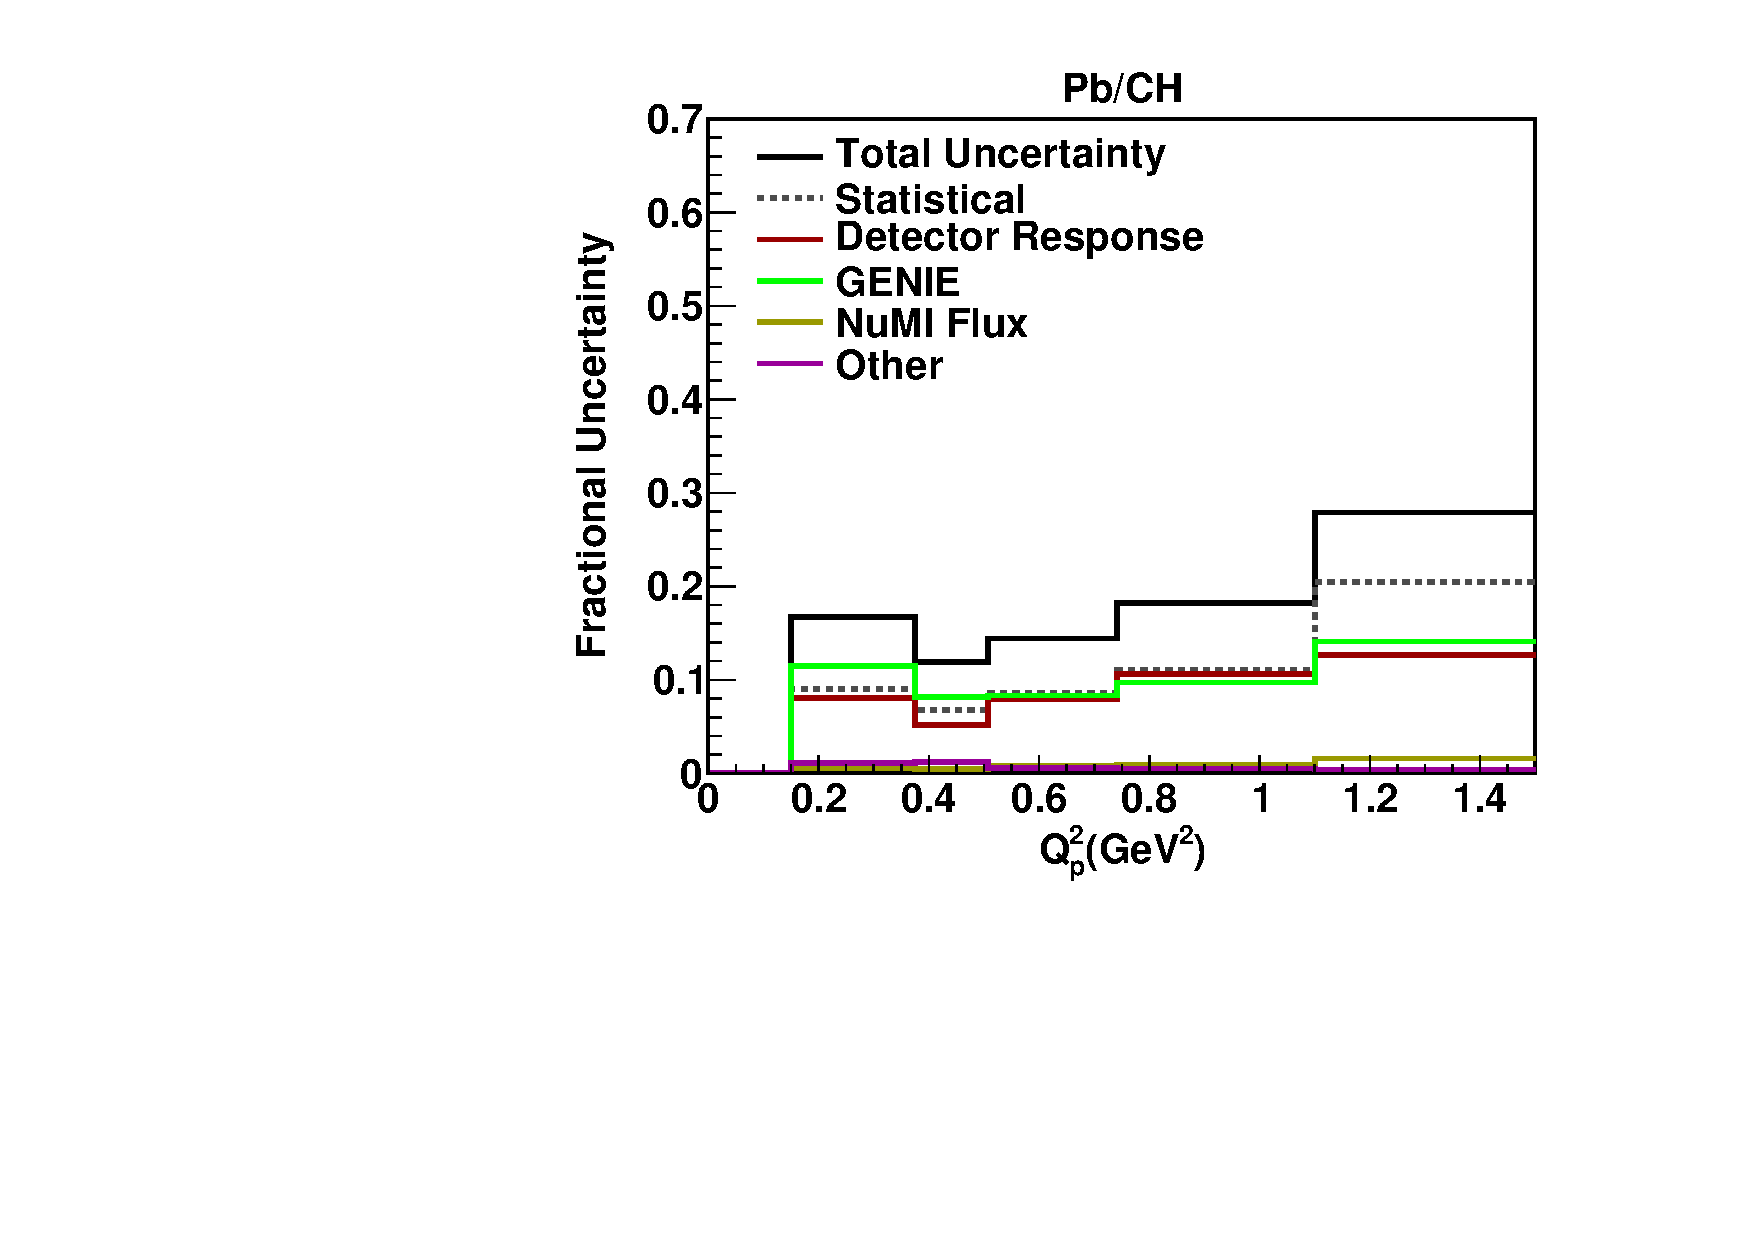
\includegraphics[trim = 0mm 4mm 10mm 2mm, width=0.48\columnwidth]{Ratio_PbError.pdf}
\caption{ Ratio of $Q^{2}_{p}$ differential cross sections on C(top-left), Fe (top-right) and Pb(bottom-left) to CH, compared to predictions from \genie and \nuwro which include 2p2h and RPA. The bottom right shows the fractional uncertainties for the $\frac{d\sigma}{dQ^{2}_{p}}$ ratio (Pb to CH), the dashed curve shows statistical uncertainty, the solid curves (color online) show systematic uncertainties each of the contributions for the systematics and black is the total uncertainty.}
\label{fig:ratios}
\end{figure}

In summary: Quasielastic-like scattering is measured for the first time, in the same neutrino beam, on nuclear targets ( C, Fe, and Pb) that span an $A$-range of 195 nucleons.
The measurements of this work reveal an $A$-dependence for the rate of quasielastic-like scattering which is not well described by current models of neutrino scattering within a nuclear medium. They will serve as benchmarks for the continued refinement of neutrino generators as is required to achieve precise delineations of mass hierarchy and CP nonconservation in the neutrino sector. 

